% Options for packages loaded elsewhere
\PassOptionsToPackage{unicode}{hyperref}
\PassOptionsToPackage{hyphens}{url}
\documentclass[
  11pt,
]{report}
\usepackage{xcolor}
\usepackage[margin=1in]{geometry}
\usepackage{amsmath,amssymb}
\setcounter{secnumdepth}{-\maxdimen} % remove section numbering
\usepackage{iftex}
\ifPDFTeX
  \usepackage[T1]{fontenc}
  \usepackage[utf8]{inputenc}
  \usepackage{textcomp} % provide euro and other symbols
\else % if luatex or xetex
  \usepackage{unicode-math} % this also loads fontspec
  \defaultfontfeatures{Scale=MatchLowercase}
  \defaultfontfeatures[\rmfamily]{Ligatures=TeX,Scale=1}
\fi
\usepackage{lmodern}
\ifPDFTeX\else
  % xetex/luatex font selection
\fi
% Use upquote if available, for straight quotes in verbatim environments
\IfFileExists{upquote.sty}{\usepackage{upquote}}{}
\IfFileExists{microtype.sty}{% use microtype if available
  \usepackage[]{microtype}
  \UseMicrotypeSet[protrusion]{basicmath} % disable protrusion for tt fonts
}{}
\makeatletter
\@ifundefined{KOMAClassName}{% if non-KOMA class
  \IfFileExists{parskip.sty}{%
    \usepackage{parskip}
  }{% else
    \setlength{\parindent}{0pt}
    \setlength{\parskip}{6pt plus 2pt minus 1pt}}
}{% if KOMA class
  \KOMAoptions{parskip=half}}
\makeatother
\usepackage{longtable,booktabs,array}
\usepackage{calc} % for calculating minipage widths
% Correct order of tables after \paragraph or \subparagraph
\usepackage{etoolbox}
\makeatletter
\patchcmd\longtable{\par}{\if@noskipsec\mbox{}\fi\par}{}{}
\makeatother
% Allow footnotes in longtable head/foot
\IfFileExists{footnotehyper.sty}{\usepackage{footnotehyper}}{\usepackage{footnote}}
\makesavenoteenv{longtable}
\usepackage{graphicx}
\makeatletter
\newsavebox\pandoc@box
\newcommand*\pandocbounded[1]{% scales image to fit in text height/width
  \sbox\pandoc@box{#1}%
  \Gscale@div\@tempa{\textheight}{\dimexpr\ht\pandoc@box+\dp\pandoc@box\relax}%
  \Gscale@div\@tempb{\linewidth}{\wd\pandoc@box}%
  \ifdim\@tempb\p@<\@tempa\p@\let\@tempa\@tempb\fi% select the smaller of both
  \ifdim\@tempa\p@<\p@\scalebox{\@tempa}{\usebox\pandoc@box}%
  \else\usebox{\pandoc@box}%
  \fi%
}
% Set default figure placement to htbp
\def\fps@figure{htbp}
\makeatother
\setlength{\emergencystretch}{3em} % prevent overfull lines
\providecommand{\tightlist}{%
  \setlength{\itemsep}{0pt}\setlength{\parskip}{0pt}}
\usepackage{bookmark}
\IfFileExists{xurl.sty}{\usepackage{xurl}}{} % add URL line breaks if available
\urlstyle{same}
\hypersetup{
  pdftitle={Multi-Turn Distributed Prompt Injection Detection},
  pdfauthor={Anonymous (under review)},
  hidelinks,
  pdfcreator={LaTeX via pandoc}}

\title{Multi-Turn Distributed Prompt Injection Detection}
\author{Anonymous (under review)}
\date{Spring 2026}

\begin{document}
\maketitle
\begin{abstract}
Single-turn prompt injection classifiers achieve high accuracy on known
attack distributions, yet they fail against multi-turn attacks that
distribute malicious intent across several conversation turns, where
each turn appears benign in isolation and the adversarial signal emerges
only from how turns relate over time. We present a dual-encoder
architecture pairing a frozen single-turn GRU encoder (2.6M parameters)
with a trainable sequence-level LSTM (27K trainable parameters) that
carries accumulated context across turns. On 73,390 single-turn samples
from eight public datasets, the Chollet heuristic correctly predicts
that a TF-IDF bag-of-bigrams classifier (F1 = 0.834) outperforms all
deep learning models, including transformers, at this data scale. On a
shared-prefix dataset of 27,180 synthetic multi-turn conversations
generated with Claude Sonnet 4.6 across four difficulty tiers, the
temporal LSTM reaches F1 = 0.837 (95\% bootstrap CI {[}0.826, 0.847{]})
and significantly outperforms turn-level max-voting by +0.131 F1 (paired
bootstrap, p \textless{} 0.001) using the same frozen encoder. Shuffling
the turn order of correctly classified attacks flips 55\% to incorrect,
the strongest evidence that the model learns genuine temporal patterns
rather than bag-of-turns features. A 66.4M-parameter concatenated
DistilBERT reaches F1 = 0.992 with 2,460x more trainable parameters; the
contribution here is not absolute accuracy but the demonstration that
temporal modeling adds significant, ordering-dependent signal beyond
per-turn classification in a 27K-parameter model deployable on
resource-constrained devices.
\end{abstract}

{
\setcounter{tocdepth}{2}
\tableofcontents
}
\section{1. Problem Statement and
Motivation}\label{problem-statement-and-motivation}

\subsection{1.1 The Problem}\label{the-problem}

Single-turn prompt injection detection achieves high accuracy on known
attack patterns. ProtectAI's DeBERTa model reaches 99\%+ F1 on published
benchmarks, yet this performance is limited to known attack
distributions. Novel attacks, adversarially crafted inputs, and
multi-turn strategies routinely evade these detectors (InjecGuard, 2024;
Vassilev, 2025). Real-world attacks against AI agent systems
increasingly distribute malicious intent across multiple conversation
turns, where each individual turn appears benign in isolation.

This is the \textbf{Crescendo attack pattern} (Russinovich et al.,
USENIX Security 2025): an attacker gradually escalates across turns,
establishing trust and context before making the exploitative request.
The \textbf{Foot-in-the-Door technique} (EMNLP 2025) similarly exploits
compliance momentum across turns. Vassilev (2025) extends Gödel's
incompleteness theorem to argue that no single-turn classifier can
theoretically detect all such attacks.

\subsection{1.2 Why Deep Learning}\label{why-deep-learning}

The multi-turn attack signal is fundamentally temporal: earlier turns
create context that later turns exploit. LSTM and GRU architectures are
designed to model exactly this type of sequential dependency through
their gating mechanisms. A bag-of-words or per-turn classifier has no
mechanism to carry forward accumulated risk state.

\subsection{1.3 Contribution}\label{contribution}

This project builds a multi-turn distributed prompt injection detection
system using a dual-encoder architecture: a frozen single-turn encoder
paired with a sequence-level LSTM that carries forward context across
turns. We evaluate on a shared-prefix dataset of 27,180 synthetic
conversations across four difficulty tiers, with bootstrap confidence
intervals and paired significance tests for all comparisons.

\begin{center}\rule{0.5\linewidth}{0.5pt}\end{center}

\section{2. Data and Preprocessing}\label{data-and-preprocessing}

\subsection{2.1 Single-Turn Datasets}\label{single-turn-datasets}

Eight HuggingFace datasets were merged:

{\def\LTcaptype{} % do not increment counter
\begin{longtable}[]{@{}
  >{\raggedright\arraybackslash}p{(\linewidth - 4\tabcolsep) * \real{0.3750}}
  >{\raggedright\arraybackslash}p{(\linewidth - 4\tabcolsep) * \real{0.3750}}
  >{\raggedright\arraybackslash}p{(\linewidth - 4\tabcolsep) * \real{0.2500}}@{}}
\toprule\noalign{}
\begin{minipage}[b]{\linewidth}\raggedright
Dataset
\end{minipage} & \begin{minipage}[b]{\linewidth}\raggedright
Samples
\end{minipage} & \begin{minipage}[b]{\linewidth}\raggedright
Type
\end{minipage} \\
\midrule\noalign{}
\endhead
\bottomrule\noalign{}
\endlastfoot
deepset/prompt-injections & 662 & Binary classification \\
xTRam1/safe-guard-prompt-injection & 10,296 & Binary classification \\
neuralchemy/Prompt-injection-dataset & 6,274 & Binary classification \\
imoxto/prompt\_injection\_cleaned\_dataset-v2 & 40,000 (subsampled from
535K) & Binary with system prompt context \\
reshabhs/SPML\_Chatbot\_Prompt\_Injection & 16,012 & Gandalf CTF
attacks \\
TrustAIRLab/in-the-wild-jailbreak-prompts (jailbreak) & 1,405 &
Real-world jailbreaks \\
TrustAIRLab/in-the-wild-jailbreak-prompts (regular) & 13,735 &
Real-world benign prompts \\
jackhhao/jailbreak-classification & 1,306 & Curated binary \\
\end{longtable}
}

After cleaning (deduplication, whitespace normalization, length
filtering), 73,390 samples remained, split 70/15/15 stratified on label:
51,373 train / 11,008 val / 11,009 test. Class balance:
\textasciitilde64\% benign / 36\% injection.

\subsection{2.2 Cleaning Pipeline}\label{cleaning-pipeline}

Nine cleaning steps applied in order: column normalization, label
normalization (0=benign, 1=injection), whitespace stripping, internal
whitespace collapse, exact deduplication, near-deduplication (lowercase
+ strip punctuation), short text removal (\textless3 tokens), long text
removal (\textgreater2048 chars), and logging.

Removals: 167 exact duplicates, 40 near-duplicates, 132 empty/short, 489
too-long.

\subsection{2.3 Synthetic Multi-Turn Data (v3
Shared-Prefix)}\label{synthetic-multi-turn-data-v3-shared-prefix}

No public dataset of multi-turn distributed attacks exists. We generated
\textbf{27,180 synthetic conversations} (18,754 train / 3,296 val /
5,130 test) using a shared-prefix architecture and the Anthropic API
(Claude Sonnet 4.6).

\textbf{Shared-prefix design}: Each conversation is generated as a
matched pair: one benign continuation and one attack continuation
branching from an identical conversational prefix. The prefix length
\emph{k} is sampled uniformly from \{3, 4, 5\} user turns. Both
continuations run for 3-5 additional turns, producing conversations of
6-9 user turns total (12-19 turns including assistant responses). This
paired structure eliminates vocabulary-level confounds in the opening
turns: a first-turn-only classifier achieves F1 = 0.35 (chance level).

\textbf{Attack strategies}:

{\def\LTcaptype{} % do not increment counter
\begin{longtable}[]{@{}
  >{\raggedright\arraybackslash}p{(\linewidth - 6\tabcolsep) * \real{0.2500}}
  >{\centering\arraybackslash}p{(\linewidth - 6\tabcolsep) * \real{0.1250}}
  >{\raggedright\arraybackslash}p{(\linewidth - 6\tabcolsep) * \real{0.2250}}
  >{\raggedright\arraybackslash}p{(\linewidth - 6\tabcolsep) * \real{0.4000}}@{}}
\toprule\noalign{}
\begin{minipage}[b]{\linewidth}\raggedright
Strategy
\end{minipage} & \begin{minipage}[b]{\linewidth}\centering
\% of Attacks
\end{minipage} & \begin{minipage}[b]{\linewidth}\raggedright
Pattern
\end{minipage} & \begin{minipage}[b]{\linewidth}\raggedright
Research Basis
\end{minipage} \\
\midrule\noalign{}
\endhead
\bottomrule\noalign{}
\endlastfoot
Fragment distribution & 45\% & Split injection across 3-5 turns,
interleaved with on-topic filler & Evasion of per-message filters \\
Gradual escalation & 25\% & Crescendo pattern, where each turn nudges
toward the attack goal & Russinovich et al.~(USENIX Security 2025) \\
Context priming & 15\% & Establish persona/authority early, exploit
later & Foot-in-the-Door (EMNLP 2025) \\
Instruction layering & 15\% & Each turn adds one constraint,
cumulatively overriding safety & Incremental constraint injection \\
\end{longtable}
}

\textbf{Difficulty tiers}: Each attack is assigned a tier (easy, medium,
hard, adversarial) controlling how aggressively the injection signal is
obscured. All splits are balanced 50/50 within each tier.

{\def\LTcaptype{} % do not increment counter
\begin{longtable}[]{@{}lrrr@{}}
\toprule\noalign{}
Tier & Train & Val & Test \\
\midrule\noalign{}
\endhead
\bottomrule\noalign{}
\endlastfoot
Easy & 5,812 & 1,002 & 1,462 \\
Medium & 5,684 & 1,000 & 1,414 \\
Hard & 5,590 & 976 & 1,394 \\
Adversarial & 1,668 & 318 & 860 \\
\end{longtable}
}

\textbf{Data quality controls}: (1) Shared-prefix pairing eliminates
early-turn confounds. (2) Validation gate: a pre-trained GRU classifier
rejects sequences where any individual turn exceeds the detection
threshold, forcing the attack signal into cross-turn patterns. (3)
Confound gate battery: seven automated checks run on 5-fold
cross-validation of training data.

\begin{figure}
\centering
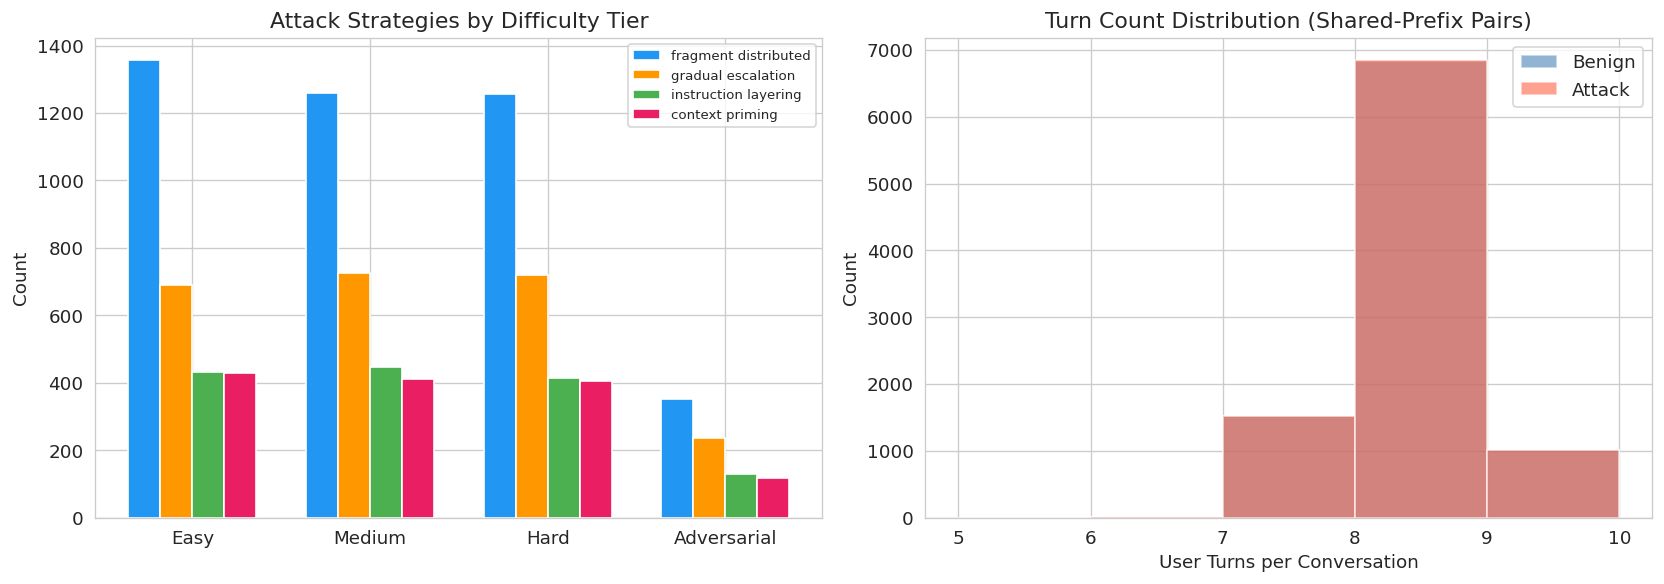
\includegraphics[width=0.95\linewidth,height=\textheight,keepaspectratio,alt={v3 shared-prefix dataset composition: difficulty-tier sizes, attack-strategy mix, and conversation-length distribution.}]{figures/v3_data_overview.png}
\caption{v3 shared-prefix dataset composition: difficulty-tier sizes,
attack-strategy mix, and conversation-length distribution.}
\end{figure}

\subsection{2.4 Tokenization}\label{tokenization}

Custom vocabulary of 20,000 tokens built from training data only. Max
sequence length: 256 tokens. OOV rate: 0.87\% on training, 1.19\% on
validation.

\subsection{2.5 Input/Output
Specification}\label{inputoutput-specification}

{\def\LTcaptype{} % do not increment counter
\begin{longtable}[]{@{}
  >{\raggedright\arraybackslash}p{(\linewidth - 8\tabcolsep) * \real{0.2500}}
  >{\raggedright\arraybackslash}p{(\linewidth - 8\tabcolsep) * \real{0.1500}}
  >{\raggedright\arraybackslash}p{(\linewidth - 8\tabcolsep) * \real{0.1750}}
  >{\raggedright\arraybackslash}p{(\linewidth - 8\tabcolsep) * \real{0.1750}}
  >{\raggedright\arraybackslash}p{(\linewidth - 8\tabcolsep) * \real{0.2500}}@{}}
\toprule\noalign{}
\begin{minipage}[b]{\linewidth}\raggedright
Variable
\end{minipage} & \begin{minipage}[b]{\linewidth}\raggedright
Type
\end{minipage} & \begin{minipage}[b]{\linewidth}\raggedright
Shape
\end{minipage} & \begin{minipage}[b]{\linewidth}\raggedright
Range
\end{minipage} & \begin{minipage}[b]{\linewidth}\raggedright
Encoding
\end{minipage} \\
\midrule\noalign{}
\endhead
\bottomrule\noalign{}
\endlastfoot
Raw text & string & variable length & n/a & Unprocessed user input \\
Token IDs (single-turn) & LongTensor & (batch, 256) & {[}0, 19999{]} &
Vocabulary lookup, post-padded with 0 \\
Token IDs (multi-turn) & LongTensor & (batch, 10, 256) & {[}0, 19999{]}
& Each turn tokenized independently \\
Turn mask & FloatTensor & (batch, 10) & \{0, 1\} & 1 = real turn, 0 =
padding \\
Model output & float & (batch, 1) & {[}0, 1{]} & Sigmoid probability of
injection \\
Label & int & scalar & \{0, 1\} & 0 = benign, 1 = injection \\
\end{longtable}
}

Raw text is lowercased and split on whitespace. Each word maps to an
integer via a vocabulary built from training data only (20,000 tokens).
Sequences shorter than 256 tokens are post-padded with zeros; sequences
longer than 256 are truncated. For multi-turn input, each turn is
encoded independently, and conversations with fewer than 10 turns are
padded with zero-vectors. The turn mask distinguishes real turns from
padding.

\subsection{2.6 Metric Selection}\label{metric-selection}

With 64\% benign and 36\% injection samples, a classifier that always
predicts ``benign'' achieves 64\% accuracy while catching zero attacks.
Accuracy rewards correct predictions on the majority class, masking
complete failure on the minority class. F1 (the harmonic mean of
precision and recall) penalizes both missed attacks (low recall) and
false alarms (low precision), making it the appropriate primary metric
for this task. The security cost asymmetry reinforces this choice: a
missed injection (false negative) can lead to system compromise, while a
false alarm (false positive) results only in a human review.

\subsection{2.7 Chollet Heuristic
Analysis}\label{chollet-heuristic-analysis}

Following Chollet (Deep Learning with Python, Chapters 11/15), the ratio
of training samples to mean words per sample (51,373 / 87.3 = 588, well
below the 1,500 threshold) predicts that bag-of-bigrams models should
outperform sequence and transformer models on single-turn data. This
prediction is empirically validated.

\begin{center}\rule{0.5\linewidth}{0.5pt}\end{center}

\section{3. Model Architecture}\label{model-architecture}

\subsection{3.1 Iteration 0: Baselines}\label{iteration-0-baselines}

TF-IDF (max 10K features, bigrams) + Logistic Regression and Random
Forest. No deep learning.

\subsection{3.2 Iterations 1-4: Single-Turn
Models}\label{iterations-1-4-single-turn-models}

{\def\LTcaptype{} % do not increment counter
\begin{longtable}[]{@{}lll@{}}
\toprule\noalign{}
Iter & Architecture & Key Feature \\
\midrule\noalign{}
\endhead
\bottomrule\noalign{}
\endlastfoot
1 & LSTM(128→64) & Random embeddings \\
2 & LSTM(100→64) & GloVe 6B 100d (frozen) \\
3 & BiLSTM(128→64) & Bidirectional + dropout (0.3, 0.5) \\
4 & BiGRU(128→64) & GRU comparison \\
\end{longtable}
}

All use: Adam optimizer, BCEWithLogitsLoss, early stopping,
ReduceLROnPlateau, gradient clipping (max\_norm=1.0).

\subsection{3.3 Iterations 4b-4c: Transformer
Comparison}\label{iterations-4b-4c-transformer-comparison}

{\def\LTcaptype{} % do not increment counter
\begin{longtable}[]{@{}
  >{\raggedright\arraybackslash}p{(\linewidth - 4\tabcolsep) * \real{0.1875}}
  >{\raggedright\arraybackslash}p{(\linewidth - 4\tabcolsep) * \real{0.4062}}
  >{\raggedright\arraybackslash}p{(\linewidth - 4\tabcolsep) * \real{0.4062}}@{}}
\toprule\noalign{}
\begin{minipage}[b]{\linewidth}\raggedright
Iter
\end{minipage} & \begin{minipage}[b]{\linewidth}\raggedright
Architecture
\end{minipage} & \begin{minipage}[b]{\linewidth}\raggedright
Key Feature
\end{minipage} \\
\midrule\noalign{}
\endhead
\bottomrule\noalign{}
\endlastfoot
4b & Custom Transformer Encoder & 2-layer, 4-head self-attention, same
vocab as LSTM \\
4c & DistilBERT (frozen body) & Transfer learning, pretrained language
model \\
\end{longtable}
}

\subsection{3.4 Iteration 5: Multi-Turn
Classifier}\label{iteration-5-multi-turn-classifier}

Dual-encoder architecture: 1. \textbf{Turn encoder} (frozen GRU from
Iter 4): encodes each turn into 32-dim vector 2. \textbf{Sequence LSTM}
(64-dim hidden): processes turn vectors temporally 3.
\textbf{Classification head}: Dense(64→32→1) with dropout

Only \textasciitilde27,000 parameters trainable (the sequence LSTM and
head). Turn encoder's 2.6M parameters are frozen.

\begin{figure}
\centering
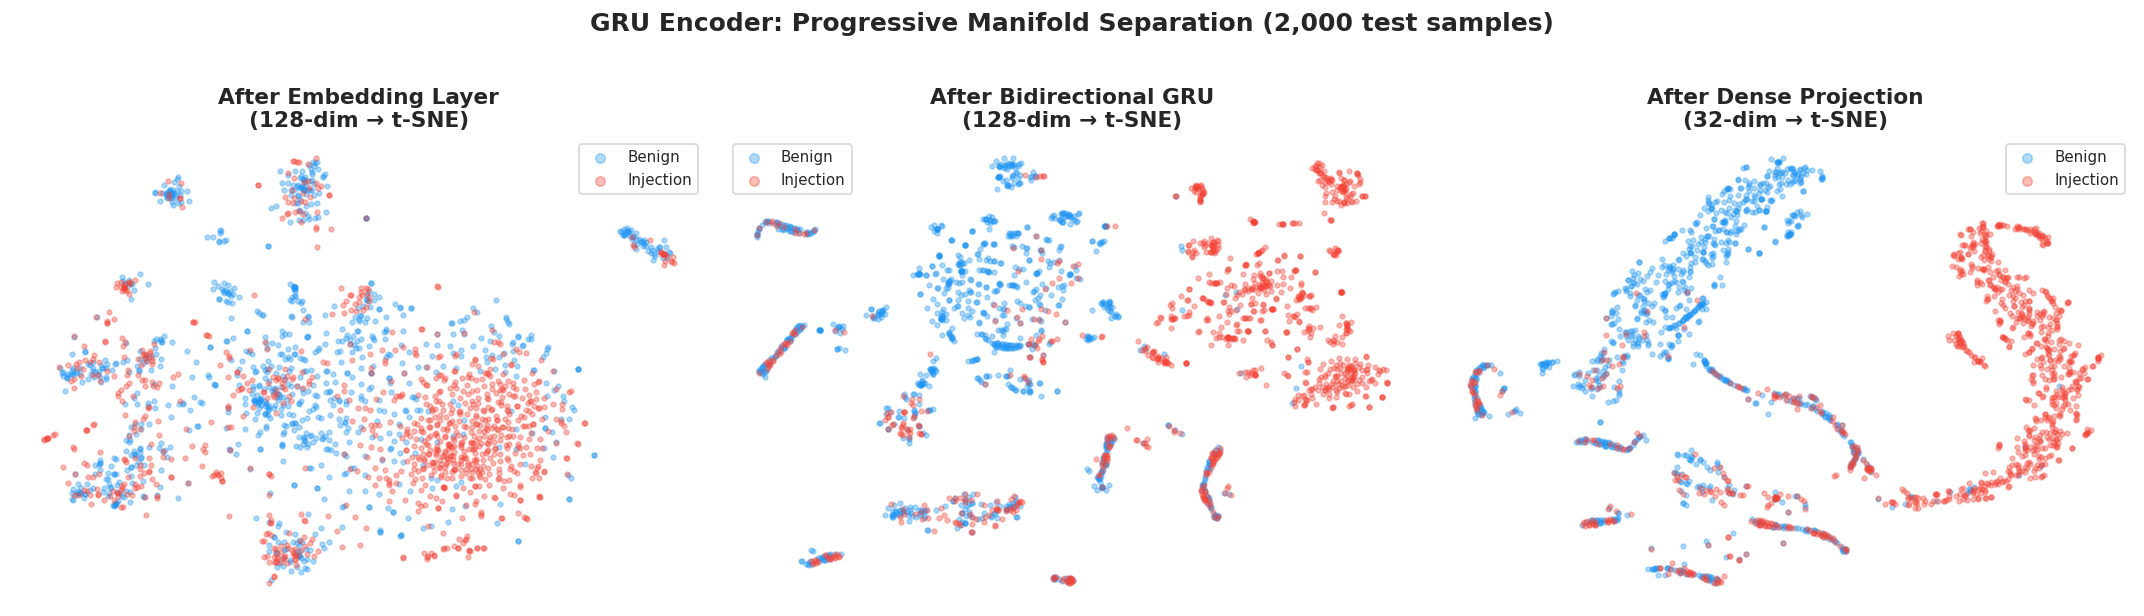
\includegraphics[width=1\linewidth,height=\textheight,keepaspectratio,alt={t-SNE of the frozen GRU turn encoder's representation space, showing progressive separation of benign and injection samples through the network.}]{figures/embedding_space_manifold.png}
\caption{t-SNE of the frozen GRU turn encoder's representation space,
showing progressive separation of benign and injection samples through
the network.}
\end{figure}

\subsection{3.5 Iteration 6: Attention}\label{iteration-6-attention}

Additive (Bahdanau) attention over sequence LSTM hidden states replaces
final-hidden-state-only classification. Each turn gets an attention
weight indicating its importance. Provides interpretability at zero
accuracy cost.

\subsection{3.6 DistilBERT Baselines}\label{distilbert-baselines}

Two transformer baselines test whether raw model capacity substitutes
for architectural design:

\begin{itemize}
\tightlist
\item
  \textbf{PM-1a: Hierarchical DistilBERT} (71.9M total, 5.5M trainable):
  Frozen DistilBERT per turn → {[}CLS{]} representations → 2-layer
  cross-turn transformer → classification head.
\item
  \textbf{PM-1b: Concatenated DistilBERT} (66.4M, all trainable): All
  turns concatenated with {[}SEP{]}, fully fine-tuned DistilBERT.
\end{itemize}

\subsection{3.7 Ablation Models}\label{ablation-models}

Five ablation experiments isolate what drives temporal detection:

{\def\LTcaptype{} % do not increment counter
\begin{longtable}[]{@{}
  >{\raggedright\arraybackslash}p{(\linewidth - 2\tabcolsep) * \real{0.4000}}
  >{\raggedright\arraybackslash}p{(\linewidth - 2\tabcolsep) * \real{0.6000}}@{}}
\toprule\noalign{}
\begin{minipage}[b]{\linewidth}\raggedright
Ablation
\end{minipage} & \begin{minipage}[b]{\linewidth}\raggedright
What It Tests
\end{minipage} \\
\midrule\noalign{}
\endhead
\bottomrule\noalign{}
\endlastfoot
A10: Turn-level voting (max, mean, top-3) & Can per-turn scoring +
aggregation match temporal modeling? \\
Shuffled turns & Is turn order informative? \\
Reversed turns & Is forward-vs-backward direction informative? \\
Mean/max pool & Does the LSTM's sequential processing add value beyond
aggregation? \\
Continuation-only / prefix-only & Which turns carry the class signal? \\
Autoencoder encoder & Does the GRU's injection-detection training
matter? \\
\end{longtable}
}

\begin{center}\rule{0.5\linewidth}{0.5pt}\end{center}

\section{4. Results}\label{results}

\subsection{4.1 Single-Turn Results}\label{single-turn-results}

{\def\LTcaptype{} % do not increment counter
\begin{longtable}[]{@{}llll@{}}
\toprule\noalign{}
Model & F1 & Accuracy & ROC-AUC \\
\midrule\noalign{}
\endhead
\bottomrule\noalign{}
\endlastfoot
Stratified random (chance) & 0.358 & 0.540 & 0.500 \\
TF-IDF + LR (Iter 0) & 0.814 & 0.878 & 0.939 \\
\textbf{TF-IDF + RF (Iter 0)} & \textbf{0.834} & \textbf{0.890} &
\textbf{0.945} \\
LSTM (Iter 1) & 0.814 & 0.877 & 0.942 \\
GloVe LSTM (Iter 2) & 0.813 & 0.881 & 0.942 \\
BiLSTM d=0.3 (Iter 3) & 0.815 & 0.884 & 0.942 \\
GRU (Iter 4) & 0.815 & 0.885 & 0.946 \\
Custom Transformer (Iter 4b) & 0.808 & 0.880 & 0.944 \\
DistilBERT frozen (Iter 4c) & 0.806 & 0.873 & 0.942 \\
\end{longtable}
}

\textbf{Encoder decision}: GRU, which offers competitive F1 with fewer
parameters than BiLSTM. Selected as the frozen turn encoder for all
multi-turn experiments.

\textbf{Chollet heuristic validated}: TF-IDF + RF achieves the highest
single-turn F1 at 0.834, confirming the prediction that at ratio 588,
simpler models outperform sequence and transformer architectures.

\subsection{4.2 Multi-Turn Results (v3 Shared-Prefix
Dataset)}\label{multi-turn-results-v3-shared-prefix-dataset}

All results below are on the v3 test set (5,130 sequences, 4 difficulty
tiers, balanced 50/50 labels). 95\% bootstrap confidence intervals from
1000 resamples.

{\def\LTcaptype{} % do not increment counter
\begin{longtable}[]{@{}
  >{\raggedright\arraybackslash}p{(\linewidth - 8\tabcolsep) * \real{0.2593}}
  >{\centering\arraybackslash}p{(\linewidth - 8\tabcolsep) * \real{0.1852}}
  >{\centering\arraybackslash}p{(\linewidth - 8\tabcolsep) * \real{0.1852}}
  >{\centering\arraybackslash}p{(\linewidth - 8\tabcolsep) * \real{0.1852}}
  >{\centering\arraybackslash}p{(\linewidth - 8\tabcolsep) * \real{0.1852}}@{}}
\toprule\noalign{}
\begin{minipage}[b]{\linewidth}\raggedright
Model
\end{minipage} & \begin{minipage}[b]{\linewidth}\centering
F1
\end{minipage} & \begin{minipage}[b]{\linewidth}\centering
95\% CI
\end{minipage} & \begin{minipage}[b]{\linewidth}\centering
AUC
\end{minipage} & \begin{minipage}[b]{\linewidth}\centering
Trainable Params
\end{minipage} \\
\midrule\noalign{}
\endhead
\bottomrule\noalign{}
\endlastfoot
Concatenated DistilBERT & 0.992 & {[}0.989, 0.994{]} & 1.000 & 66.4M \\
Hierarchical DistilBERT & 0.976 & {[}0.971, 0.980{]} & 0.998 & 5.5M \\
Continuation-only LSTM & 0.846 & {[}0.835, 0.856{]} & 0.923 & 27K \\
Autoencoder encoder & 0.845 & {[}0.834, 0.856{]} & 0.922 & 27K \\
Iter 6 (+attention) & 0.837 & {[}0.825, 0.848{]} & 0.921 & 29K \\
\textbf{Iter 5 (temporal LSTM)} & \textbf{0.837} & \textbf{{[}0.826,
0.847{]}} & \textbf{0.919} & \textbf{27K} \\
Reversed turns & 0.833 & {[}0.821, 0.844{]} & 0.916 & 27K \\
Shuffled turns & 0.760 & {[}0.748, 0.772{]} & 0.849 & 27K \\
Mean pool & 0.755 & {[}0.743, 0.768{]} & 0.839 & 27K \\
A10 top-3-mean voting & 0.727 & n/a & n/a & 0 \\
Max pool & 0.719 & {[}0.705, 0.733{]} & 0.819 & 27K \\
A10 max-vote & 0.706 & n/a & n/a & 0 \\
Prefix-only & 0.667 & {[}0.655, 0.679{]} & 0.500 & 27K \\
Cosine baseline & 0.612 & {[}0.596, 0.627{]} & 0.642 & 0 \\
A10 mean-vote & 0.231 & n/a & n/a & 0 \\
\end{longtable}
}

\begin{figure}
\centering
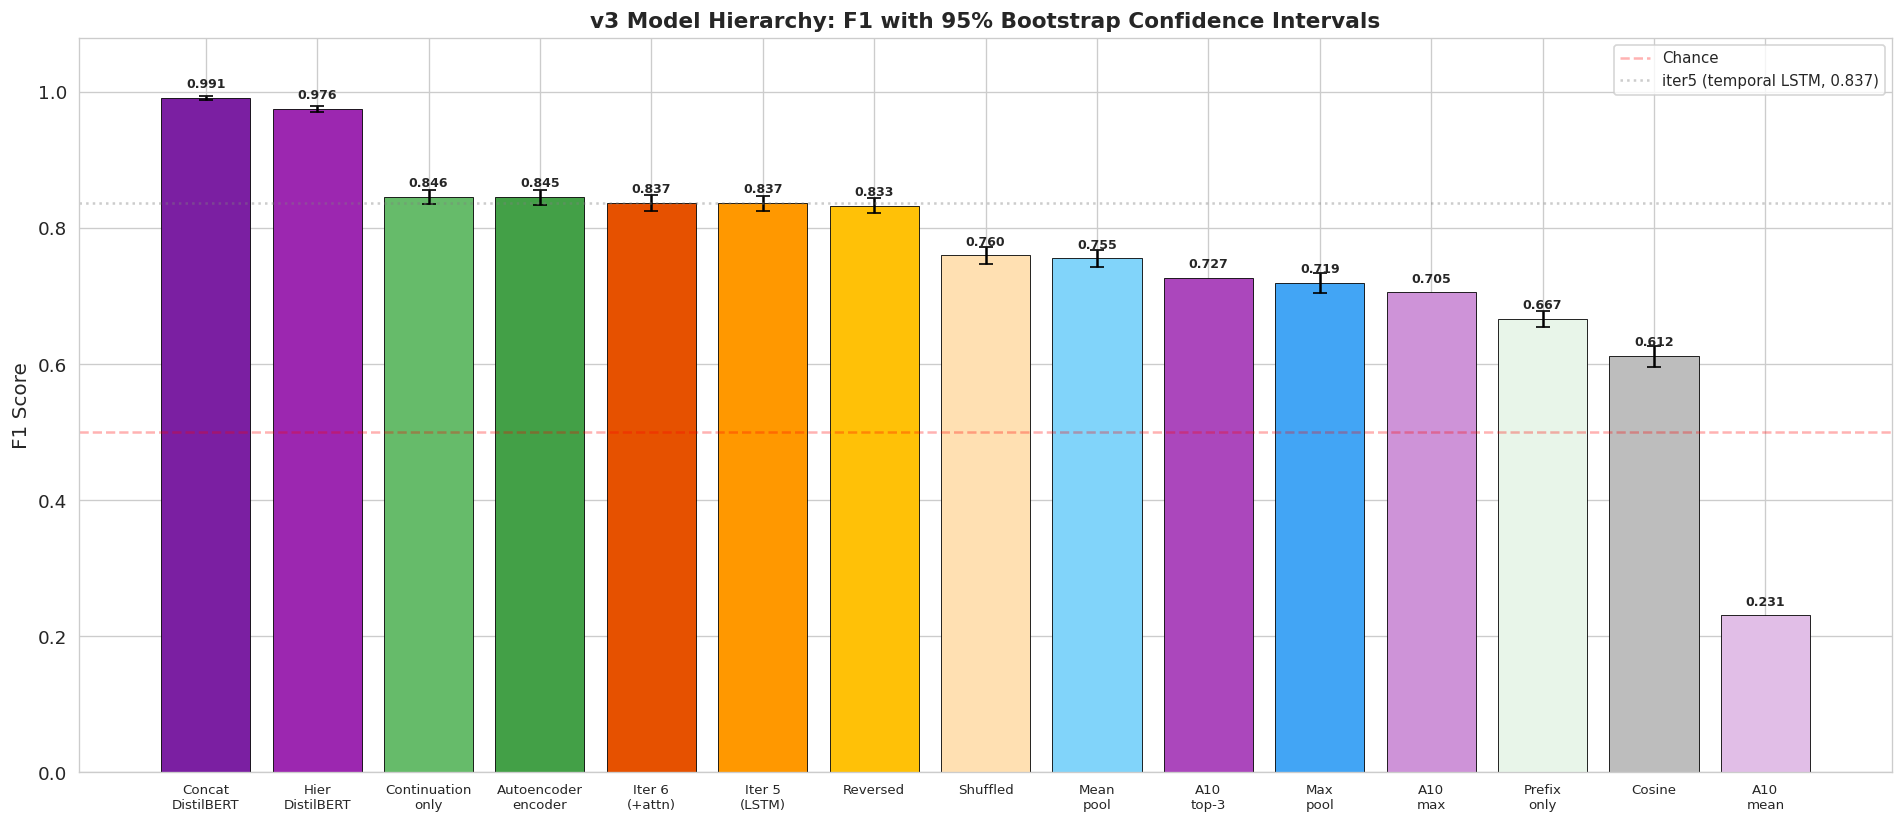
\includegraphics[width=0.9\linewidth,height=\textheight,keepaspectratio,alt={Model hierarchy on the v3 shared-prefix test set (5,130 sequences) with 95\% bootstrap confidence intervals from 1000 resamples.}]{figures/v3_model_hierarchy.png}
\caption{Model hierarchy on the v3 shared-prefix test set (5,130
sequences) with 95\% bootstrap confidence intervals from 1000
resamples.}
\end{figure}

\subsection{4.3 Per-Tier Breakdown}\label{per-tier-breakdown}

{\def\LTcaptype{} % do not increment counter
\begin{longtable}[]{@{}lcccr@{}}
\toprule\noalign{}
Tier & iter5 F1 & iter6 F1 & DistilBERT-concat F1 & n \\
\midrule\noalign{}
\endhead
\bottomrule\noalign{}
\endlastfoot
Easy & 0.872 & 0.876 & 0.994 & 1,462 \\
Medium & 0.828 & 0.832 & 0.991 & 1,414 \\
Hard & 0.828 & 0.830 & 0.994 & 1,394 \\
Adversarial & 0.802 & 0.786 & 0.985 & 860 \\
\end{longtable}
}

\begin{figure}
\centering
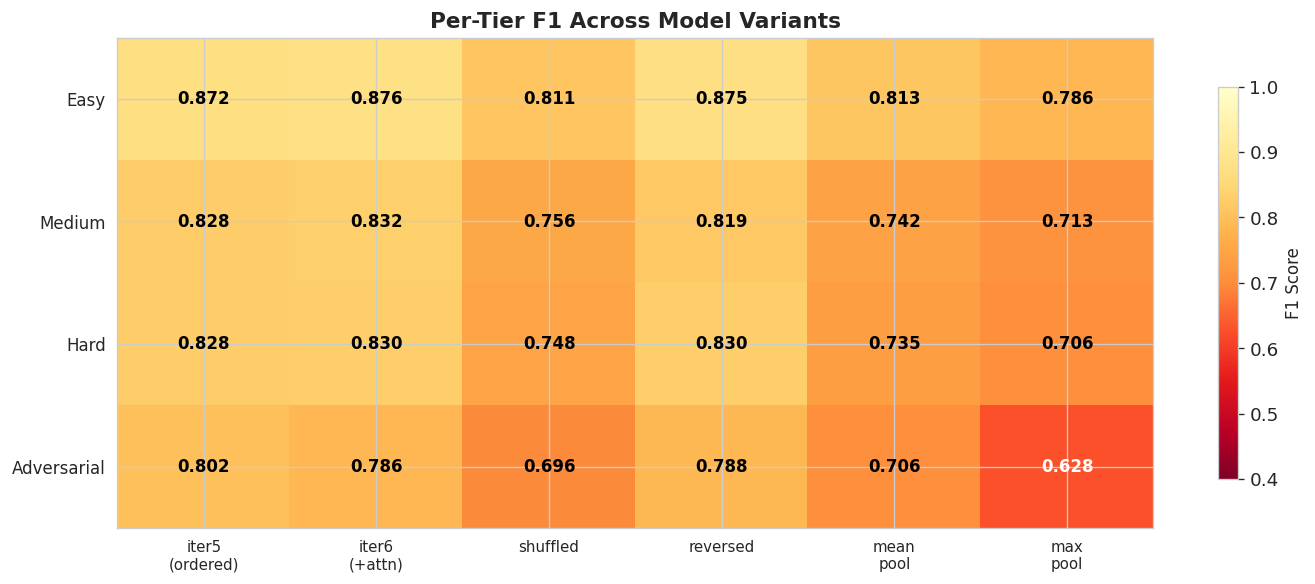
\includegraphics[width=0.9\linewidth,height=\textheight,keepaspectratio,alt={Per-tier F1 across model variants. The difficulty ordering (easy to adversarial) is stable across architectures, confirming the tiers measure a model-independent property.}]{figures/v3_tier_variant_heatmap.png}
\caption{Per-tier F1 across model variants. The difficulty ordering
(easy to adversarial) is stable across architectures, confirming the
tiers measure a model-independent property.}
\end{figure}

\subsection{4.4 Statistical
Significance}\label{statistical-significance}

Paired one-sided bootstrap tests (1000 resamples):

{\def\LTcaptype{} % do not increment counter
\begin{longtable}[]{@{}lcc@{}}
\toprule\noalign{}
Comparison & F1 Diff & p-value \\
\midrule\noalign{}
\endhead
\bottomrule\noalign{}
\endlastfoot
iter5 \textgreater{} A10 max-vote & +0.131 & \textless{} 0.001 \\
iter5 \textgreater{} A10 top-3-mean & +0.110 & \textless{} 0.001 \\
iter5 \textgreater{} shuffled turns & +0.077 & \textless{} 0.001 \\
iter6 \textgreater{} iter5 & +0.000 & 0.453 (n.s.) \\
DistilBERT-concat \textgreater{} iter5 & +0.155 & \textless{} 0.001 \\
\end{longtable}
}

\subsection{4.5 Turn-Order Sensitivity}\label{turn-order-sensitivity}

Shuffling the turns of correctly classified attack sequences: 55\% flip
from correct to incorrect. Ordered F1 = 0.837 → shuffled F1 = 0.489 (on
the originally-correct subset). Flip rate is uniform across tiers
(54-56\%).

\begin{figure}
\centering
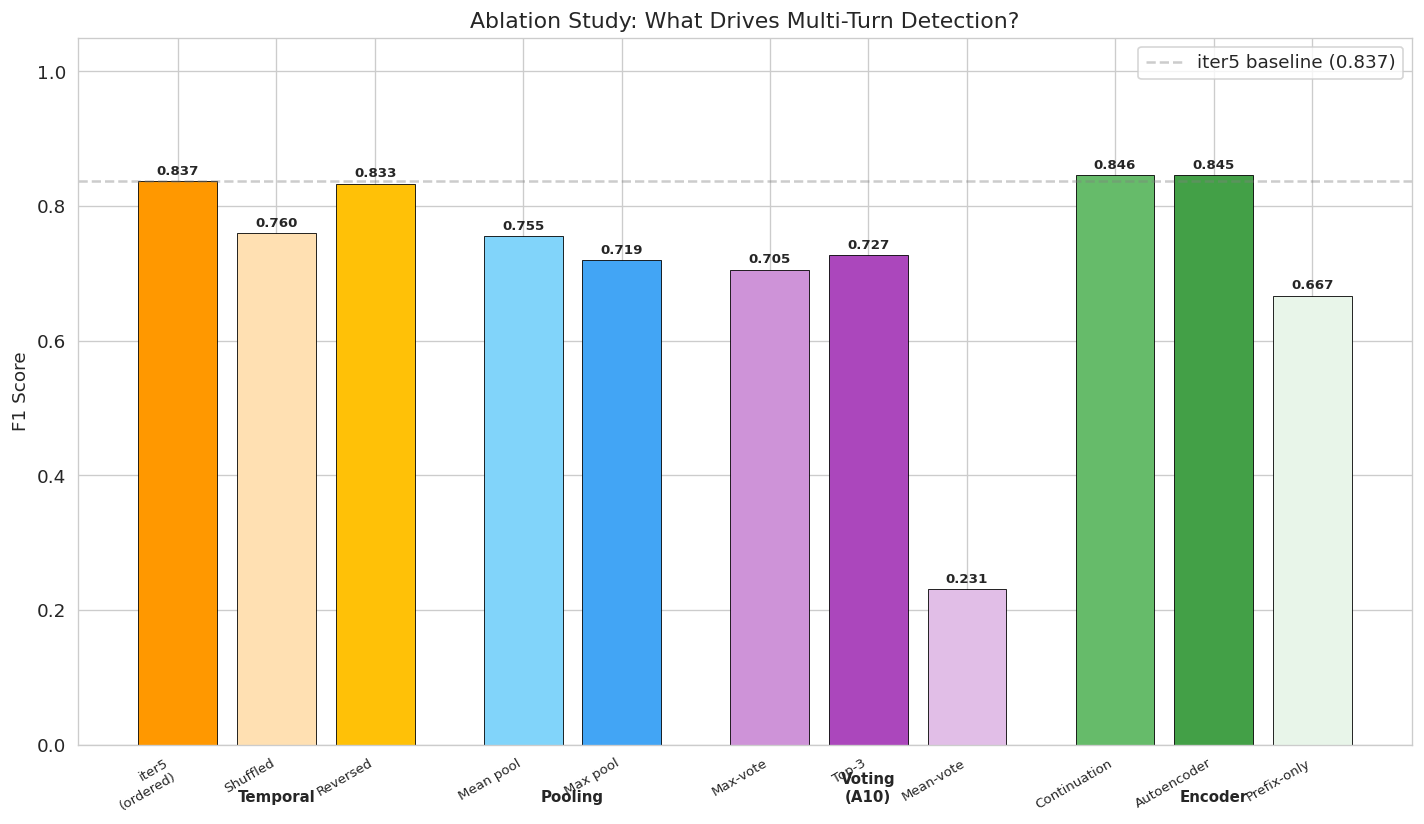
\includegraphics[width=0.9\linewidth,height=\textheight,keepaspectratio,alt={Turn-order and pooling ablations: ordered baseline versus shuffled, reversed, mean pool, max pool, and prefix-only. Shuffling drops F1 by 0.077 (p \textless{} 0.001).}]{figures/v3_ablation_summary.png}
\caption{Turn-order and pooling ablations: ordered baseline versus
shuffled, reversed, mean pool, max pool, and prefix-only. Shuffling
drops F1 by 0.077 (p \textless{} 0.001).}
\end{figure}

\subsection{4.6 Per-Strategy Breakdown}\label{per-strategy-breakdown}

{\def\LTcaptype{} % do not increment counter
\begin{longtable}[]{@{}lccc@{}}
\toprule\noalign{}
Strategy & iter5 F1 & iter6 F1 & n (test) \\
\midrule\noalign{}
\endhead
\bottomrule\noalign{}
\endlastfoot
Fragment distribution & 0.776 & 0.787 & 1,160 \\
Gradual escalation & 0.676 & 0.681 & 669 \\
Context priming & 0.628 & 0.650 & 372 \\
Instruction layering & 0.605 & 0.612 & 364 \\
\end{longtable}
}

\begin{figure}
\centering
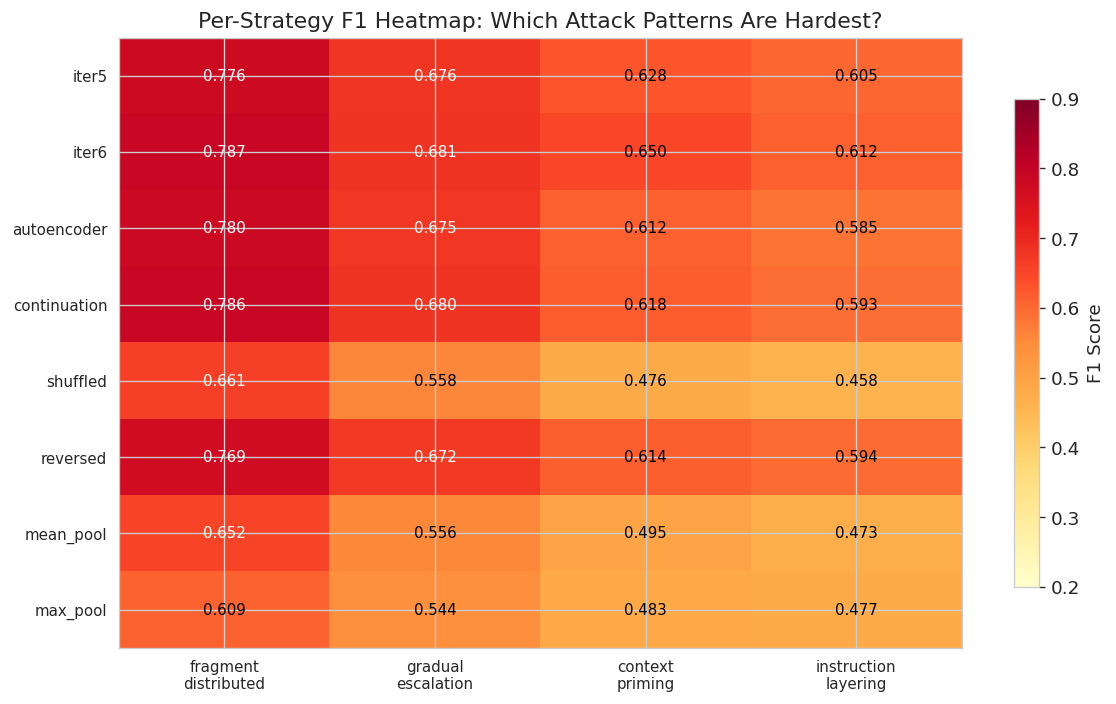
\includegraphics[width=0.9\linewidth,height=\textheight,keepaspectratio,alt={Per-strategy F1 for the temporal models. Fragment distribution is easiest to detect; instruction layering is hardest, consistent with its smoother cumulative signal.}]{figures/v3_strategy_heatmap.png}
\caption{Per-strategy F1 for the temporal models. Fragment distribution
is easiest to detect; instruction layering is hardest, consistent with
its smoother cumulative signal.}
\end{figure}

\subsection{4.7 Confound Gate Analysis}\label{confound-gate-analysis}

Seven gates run on 5-fold cross-validation of training data:

{\def\LTcaptype{} % do not increment counter
\begin{longtable}[]{@{}lccc@{}}
\toprule\noalign{}
Gate & F1 (5-fold mean) & Threshold & Result \\
\midrule\noalign{}
\endhead
\bottomrule\noalign{}
\endlastfoot
First-turn only & 0.354 & \textless{} 0.58 & PASS \\
Conversation length & 0.482 & \textless{} 0.55 & PASS \\
Max-vote BoW & 0.684 & \textless{} 0.70 & PASS \\
Unigram BoW & 0.938 & \textless{} 0.60 & FAIL \\
Bigram BoW & 0.945 & \textless{} 0.65 & FAIL \\
Last-turn only & 0.963 & \textless{} 0.65 & FAIL \\
Mean-vote BoW & 0.926 & \textless{} 0.65 & FAIL \\
\end{longtable}
}

The passing gates confirm the shared-prefix design eliminates early-turn
and length confounds. The failing gates indicate that vocabulary
differences persist in post-branch turns. The turn-order sensitivity
analysis (55\% flip rate) demonstrates that the temporal LSTM relies on
ordering information that BoW classifiers cannot exploit.

\begin{center}\rule{0.5\linewidth}{0.5pt}\end{center}

\begin{figure}
\centering
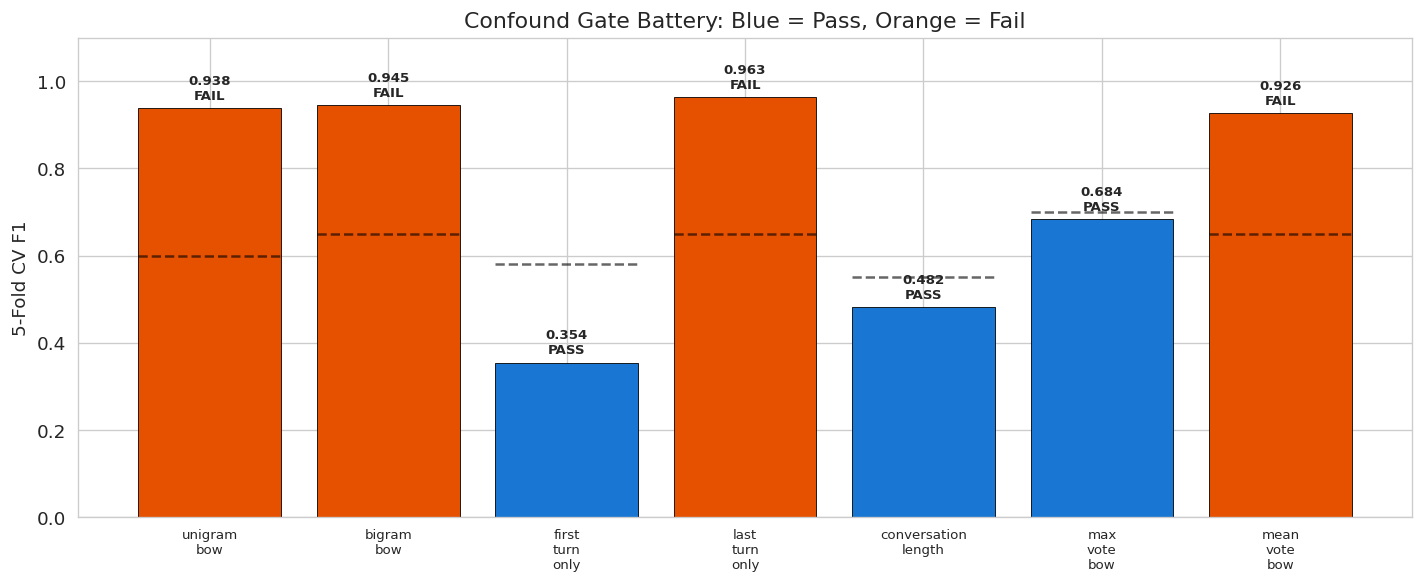
\includegraphics[width=0.85\linewidth,height=\textheight,keepaspectratio,alt={Confound gate battery run on 5-fold cross-validation of training data. Passing gates (first-turn, length, max-vote BoW) confirm the shared-prefix design; failing vocabulary gates motivate the turn-order analysis.}]{figures/v3_confound_gates.png}
\caption{Confound gate battery run on 5-fold cross-validation of
training data. Passing gates (first-turn, length, max-vote BoW) confirm
the shared-prefix design; failing vocabulary gates motivate the
turn-order analysis.}
\end{figure}

\section{5. Discussion}\label{discussion}

\subsection{5.1 Why Temporal Modeling
Works}\label{why-temporal-modeling-works}

The dual-encoder architecture succeeds because it separates two
concerns: 1. \textbf{What does each turn say?} (turn encoder, frozen,
compressing to 32-dim) 2. \textbf{How do turns relate over time?}
(sequence LSTM, which learns temporal patterns)

The turn-level voting gap (+0.131 F1 over max-vote, p \textless{} 0.001)
demonstrates that independent per-turn scoring cannot recover the
cross-turn signal. The shuffled-turns gap (+0.077 F1, p \textless{}
0.001) confirms that turn order carries genuine information. These two
results together establish that the LSTM learns temporal relationships,
not bag-of-turns features.

\begin{figure}
\centering
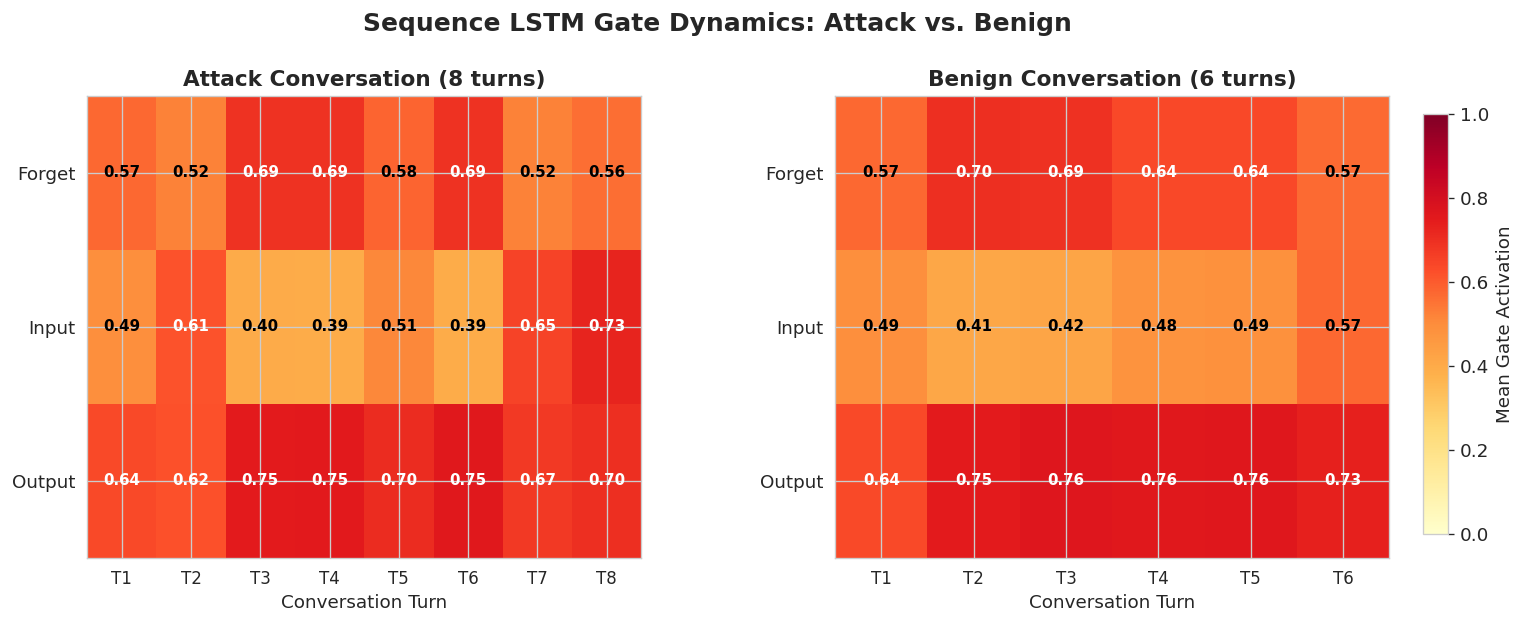
\includegraphics[width=0.9\linewidth,height=\textheight,keepaspectratio,alt={LSTM forget, input, and output gate activations across conversation turns for representative attack and benign sequences. The forget gate drops at the divergence point in attacks.}]{figures/gate_activations_heatmap.png}
\caption{LSTM forget, input, and output gate activations across
conversation turns for representative attack and benign sequences. The
forget gate drops at the divergence point in attacks.}
\end{figure}

\subsection{5.2 The DistilBERT Question}\label{the-distilbert-question}

Concatenated DistilBERT achieves F1 = 0.992 with 66.4M trainable
parameters versus our 0.837 with 27K, a 2,460x parameter ratio. This gap
has two interpretations:

The DistilBERT models have full text access and can exploit both
temporal and vocabulary signals, including the residual vocabulary
differences that the confound gates flagged. Our model operates in a
32-dimensional embedding space where vocabulary is compressed away.

The comparison that matters is not ``does our model beat DistilBERT''
(it does not) but ``does temporal modeling add value beyond per-turn
classification'' (it does, significantly). The 27K-parameter temporal
model is deployable on resource-constrained devices where DistilBERT is
impractical.

\begin{figure}
\centering
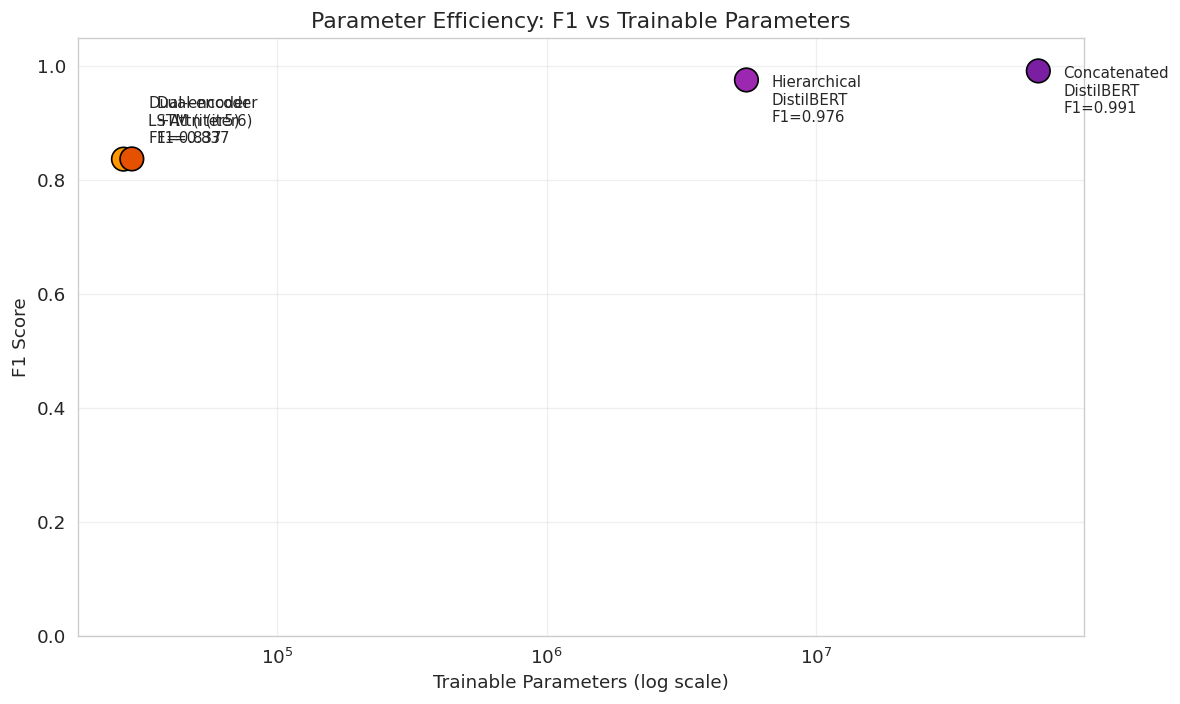
\includegraphics[width=0.8\linewidth,height=\textheight,keepaspectratio,alt={F1 versus trainable parameter count. The 27K-parameter temporal LSTM and 66.4M-parameter concatenated DistilBERT bound the accuracy-efficiency Pareto frontier.}]{figures/v3_param_efficiency.png}
\caption{F1 versus trainable parameter count. The 27K-parameter temporal
LSTM and 66.4M-parameter concatenated DistilBERT bound the
accuracy-efficiency Pareto frontier.}
\end{figure}

\subsection{5.3 What the Autoencoder Ablation
Reveals}\label{what-the-autoencoder-ablation-reveals}

Replacing the injection-trained GRU encoder with a
reconstruction-trained autoencoder yields F1 = 0.845, slightly exceeding
the primary model (F1 = 0.837). This result indicates that the sequence
LSTM drives temporal detection regardless of whether the turn encoder
was trained for injection classification. The GRU's injection-detection
expertise does not transfer to the multi-turn task in a measurable way.

Two explanations are plausible. The injection-trained GRU's
32-dimensional output may already compress away the features most useful
for temporal analysis, retaining only an ``injection-likeness'' score
that the sequence LSTM must work around rather than with. Alternatively,
the autoencoder's reconstruction objective may preserve richer turn
representations that happen to be equally informative for temporal
pattern recognition. Distinguishing these explanations would require
probing the information content of each encoder's representations, which
we leave as future work.

This finding tempers the dual-encoder narrative. The architecture's
value lies in the frozen-encoder-plus-temporal-LSTM decomposition
itself, not in the specific training objective of the encoder. Any
encoder that produces meaningful fixed-dimensional turn representations
appears sufficient for temporal detection.

\subsection{5.4 Limitations}\label{limitations}

\begin{itemize}
\tightlist
\item
  \textbf{Synthetic data}: All conversations generated by Claude Sonnet
  4.6. Performance on naturally occurring multi-turn attacks is unknown.
\item
  \textbf{Residual vocabulary confounds}: BoW classifiers achieve F1
  \textgreater{} 0.93 on training data. The temporal signal operates on
  top of this confound.
\item
  \textbf{Single model family}: Cross-model generalization (attacks
  generated by GPT-4, Gemini, open-weight models) is untested.
\item
  \textbf{Fixed conversation length}: 6-9 user turns. Behavior on 20+
  turn conversations is untested.
\item
  \textbf{English only}: Non-English injection patterns are not
  represented.
\end{itemize}

\subsection{5.5 Future Work}\label{future-work}

\begin{enumerate}
\def\labelenumi{\arabic{enumi}.}
\tightlist
\item
  \textbf{Cross-domain transfer}: Test on multi-turn attack data from
  different domains
\item
  \textbf{Real-world validation}: Deploy as a secondary filter behind
  production AI systems
\item
  \textbf{Online detection}: Classify after each new turn for streaming
  inference
\item
  \textbf{Formal safety analysis}: Investigate whether LSTM hidden-state
  trajectories satisfy the Markov property for connection to formal
  verification approaches
\item
  \textbf{Longer contexts}: Extend to 20-50 turn conversations common in
  production
\end{enumerate}

\begin{center}\rule{0.5\linewidth}{0.5pt}\end{center}

\section{6. Reproducibility}\label{reproducibility}

\begin{itemize}
\tightlist
\item
  \textbf{Seed}: 42 for all random operations (Python, NumPy, PyTorch,
  cuDNN)
\item
  \textbf{Platform}: NVIDIA Jetson Orin AGX, PyTorch 2.8.0, Python 3.12
\item
  \textbf{Data}: Single-turn from HuggingFace (Apache 2.0 / MIT).
  Multi-turn generated via Anthropic API.
\item
  \textbf{Code}: Full source in \texttt{src/}, evaluation in
  \texttt{scripts/}, results in \texttt{results/v3\_evaluation/}
\item
  \textbf{Hardware}: 64GB RAM, Ampere GPU (sm\_87), CUDA 12.6. Training
  run on RunPod A100.
\item
  \textbf{Statistical methods}: 1000-sample bootstrap for CIs, paired
  one-sided bootstrap for significance tests.
\end{itemize}

All model weights, metrics, predictions (.npz), and plots saved to
\texttt{models/} and \texttt{results/} directories.

\end{document}
